

\tikzset{every picture/.style={line width=0.75pt}} %set default line width to 0.75pt        

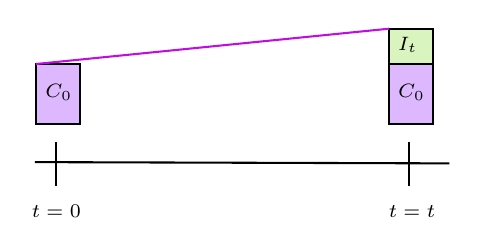
\begin{tikzpicture}[x=0.75pt,y=0.75pt,yscale=-1,xscale=1]
%uncomment if require: \path (0,300); %set diagram left start at 0, and has height of 300

%Straight Lines [id:da001] - Main timeline
\draw    (198,173) -- (397.68,173.61) ;
%Straight Lines [id:da002] - Vertical tick at t=0
\draw    (208.2,163.27) -- (208.2,184.27) ;
%Straight Lines [id:da003] - Vertical tick at t=t
\draw    (378.2,163.27) -- (378.2,184.27) ;
%Shape: Rectangle [id:dp001] - Capital at t=0
\draw  [fill={rgb, 255:red, 144; green, 19; blue, 254 }  ,fill opacity=0.3 ] (198.53,125.73) -- (219.81,125.73) -- (219.81,154.73) -- (198.53,154.73) -- cycle ;
%Shape: Rectangle [id:dp002] - Capital at t=t
\draw  [fill={rgb, 255:red, 144; green, 19; blue, 254 }  ,fill opacity=0.3 ] (368.53,125.73) -- (389.81,125.73) -- (389.81,154.73) -- (368.53,154.73) -- cycle ;
%Shape: Rectangle [id:dp003] - Interest at t=t
\draw  [fill={rgb, 255:red, 184; green, 233; blue, 134 }  ,fill opacity=0.52 ] (368.53,108.73) -- (389.81,108.73) -- (389.81,125.53) -- (368.53,125.53) -- cycle ;
%Straight Lines [id:da004] - Arrow showing interest growth
\draw [color={rgb, 255:red, 189; green, 16; blue, 224 }  ,draw opacity=1 ]   (198.53,125.73) -- (368.53,108.73) ;

% Text Node
\draw (195,192.4) node [anchor=north west][inner sep=0.75pt]  [font=\scriptsize]  {$t=0$};
% Text Node
\draw (367,192.4) node [anchor=north west][inner sep=0.75pt]  [font=\scriptsize]  {$t=t$};
% Text Node
\draw (201.53,133.93) node [anchor=north west][inner sep=0.75pt]  [font=\scriptsize]  {$C_{0}$};
% Text Node
\draw (371.53,133.93) node [anchor=north west][inner sep=0.75pt]  [font=\scriptsize]  {$C_{0}$};
% Text Node
\draw (371.53,111.13) node [anchor=north west][inner sep=0.75pt]  [font=\scriptsize]  {$I_{t}$};


\end{tikzpicture}
